\section{}
% A rectangular plate is subjected to uniform tensile stress σ along its upper and lower edges as
% shown in Fig. 2. Determine the displacements u and v in terms of x, y, and material properties
% (E, ν) using Eqn. (2) and the appropriate conditions at the origin.
% Figure 2: A rectangular plate
% εx = ∂u
% ∂x, εy = ∂v
% ∂y (2a)
% γxy = αx − αy = ∂u
% ∂y + ∂v
% ∂x (2b)
% 3

A rectangular plate is subjected to uniform tensile stress $\sigma$ along its upper and 
lower edges as shown in Fig. \ref{fig:Q3}. Determine the displacements $u$ and $v$ in terms 
of $x$, $y$, and material properties ($E$, $\nu$) using Eqns. (\ref{eq:Q3Strain}) and (\ref{eq:Q3Shear}) and the appropriate 
conditions at the origin.

\begin{figure}[h]
    \centering
    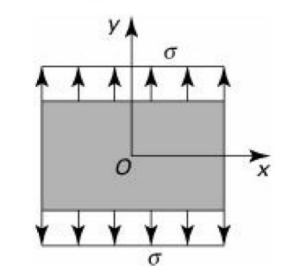
\includegraphics[width=0.5\linewidth]{Questions/Figures/Q3ProblemDiagram.png}
    \caption{Rectangular plate subjected to uniform tensile stress.}
    \label{fig:Q3}
\end{figure}

\begin{align}
    \epsilon_x &= \frac{\nabla u}{\nabla x}, \;\; \epsilon_y = \frac{\nabla v}{\nabla y} \label{eq:Q3Strain} \\
    \gamma_{xy} &= \alpha_x - \alpha_y = \frac{\nabla u}{\nabla y} + \frac{\nabla v}{\nabla x} \label{eq:Q3Shear}
\end{align}

